\section{File Storage}
\label{sec:data_structure}
The file storage is organized into three major directories, {\em RAW}, {\em OSG}
and {\em POTREE}. Their structure and the nomenclature is described in the coming
sections as well as the scripts to manipulate their content.

\subsection{File storage structure}
\label{sec:descriptiondata}
The raw data is \textbf{only} stored in the Via Appia Linux server. Through a python
script, called \textit{createosgdata.py}, raw data is converted to OSG data. Another
script, called \textit{CreatePotreeConfig.py}, converts the raw data into Potree
internal format. More details about these two scripts can be found in Section~\ref{sec:generateosg}
and Section~\ref{sec:generatePotree}. 

These two scripts pick raw data from \textit{/home/vadata/DATA/RAW}. After the data
generation, the OSG data is stored in \textit{/home/vadata/DATA/OSG} and POTREE data
is stored in \textit{/home/vadata/DATA/POTREE}, c.f., Figure~\ref{fig:directory_structure_overview}.

\begin{figure}[!ht] \centering
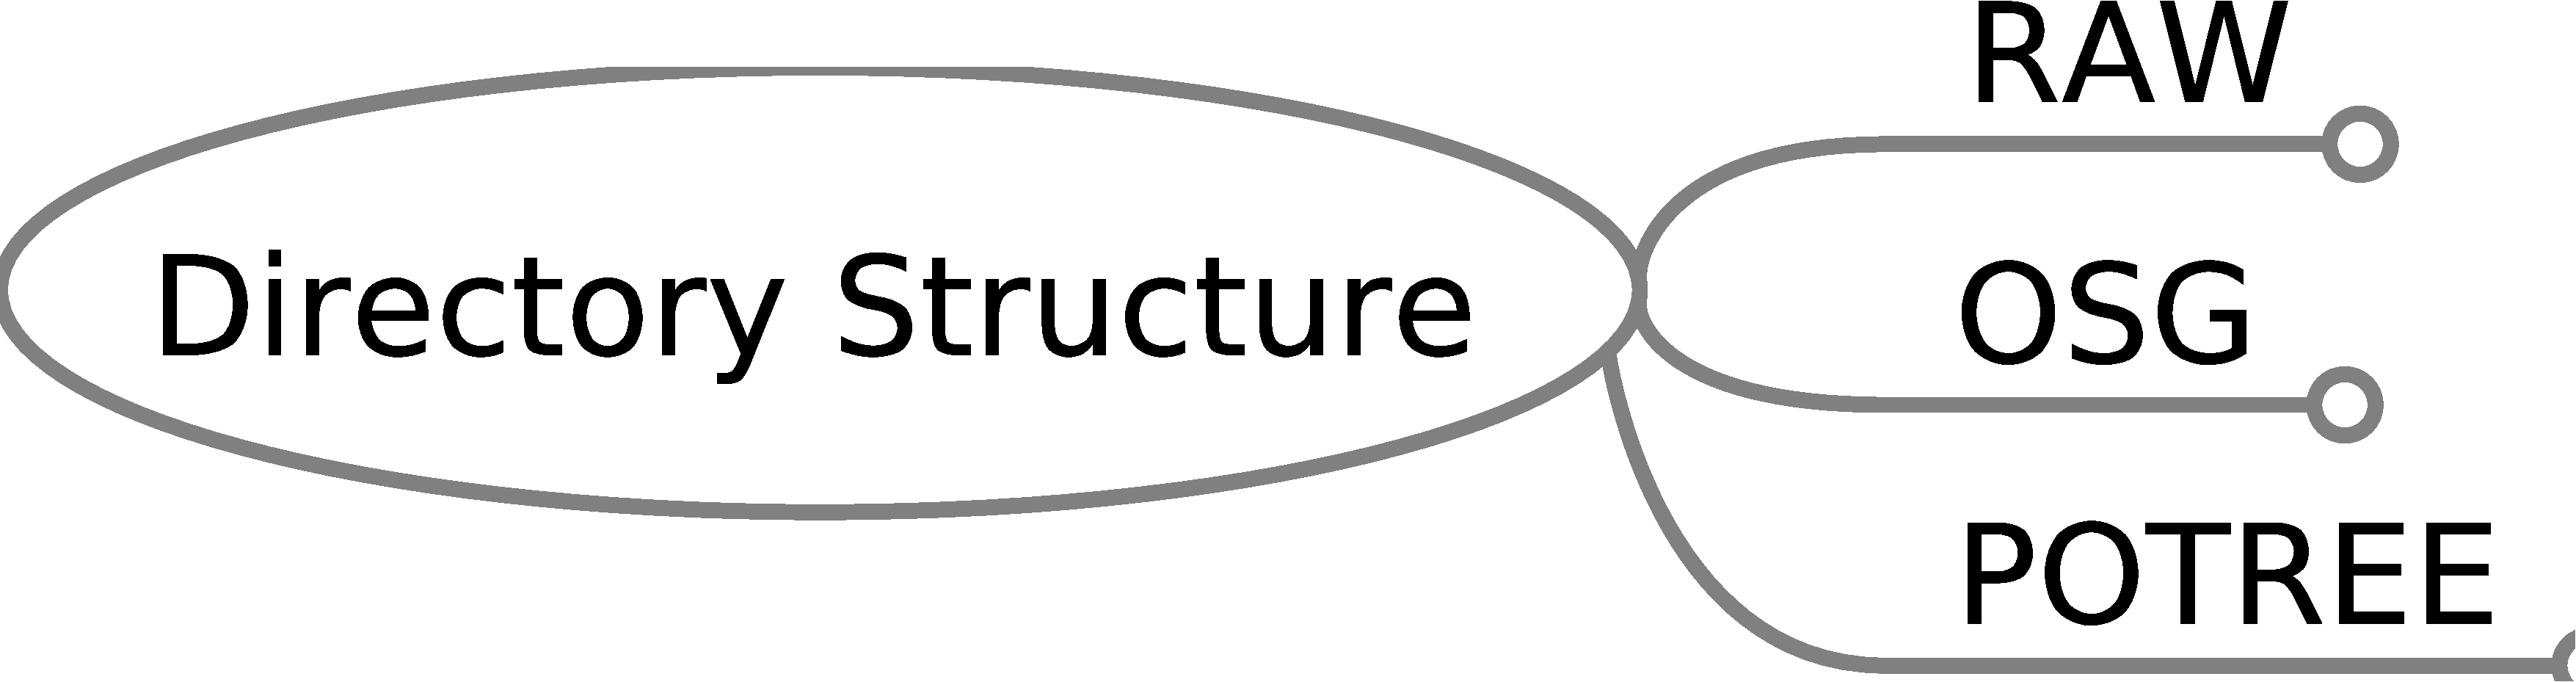
\includegraphics[width=0.4\textwidth]{fig/data_structure/directory_structure_overview}
\caption{Overview of the data structure}
\label{fig:directory_structure_overview} \end{figure}

\subsubsection{Nomenclature}
The directories and files name follow a specific nomenclature which describes a
bit their content. Such information is then used by the data preparation scripts
to locate the required data and also by the system to serve the user requests.
These rules apply to all directories and files under raw, OSG and Potree data
directories.

Under the raw data directory there is a sub-directory for point clouds, meshes
and pictures. Each of them have a sub-directory for backgrounds called \textit{BACK}
and one for sites called \textit{SITE}. For backgrounds, the subdirectory contains
different folders with point clouds for each background. For sites, the subdirectory
contains a separate folder for each site. For example, \textit{MESH/SITE/CURR/S162}
could contain two folders called \textit{162\_curr\_1} and \textit{162\_curr\_2}.

Point Clouds and meshes can have two types of background and sites: (a) current
representations, and (b) archeological reconstructions. They are stored in respectively
\textit{CURR} and \textit{RCH\_REC}. For pictures the sub-division has a different
nomenclature. The subdivision is made between (a) pictures of the current state of
the sites, and (b) historical pictures and paintings. These are stored in respectively
\textit{CURR} and \textit{HIST}.

The LAS files contained in each site sub-folder may have been pre-aligned through a
third party tool such as CloudCompare. In that case the LAS file name must contain
\textbf{*\_ALIGNED\_\textit{BGNAME}*} where \textit{BGNAME} is the background name
(as contained in the folder \textit{PC/BACK/}).

Some point clouds generation tools store the color information in 8 bits instead of
the usual 16 bits. In that case the folder name must be \textbf{*\_8BC}. The effect
of having an undeclared LAS file with 8 bit color is that the converted data will be
black and white. Note that these properties are cumulative, for example
\textit{S162\_ALIGNED\_DRIVE\_1\_V3\_8BC} is a valid name for a folder containing
a LAS file with 8 bit color information and aligned points.

This hierarchy of folders and nomenclature for the raw data, as shown in Figure~\ref{fig:directory_structure_overview_raw},
is also used for the OSG directories, Figure~\ref{fig:directory_structure_overview_osg},
and for the Potree directories, Figure~\ref{fig:directory_structure_overview_potree}.

\begin{figure}[] \centering
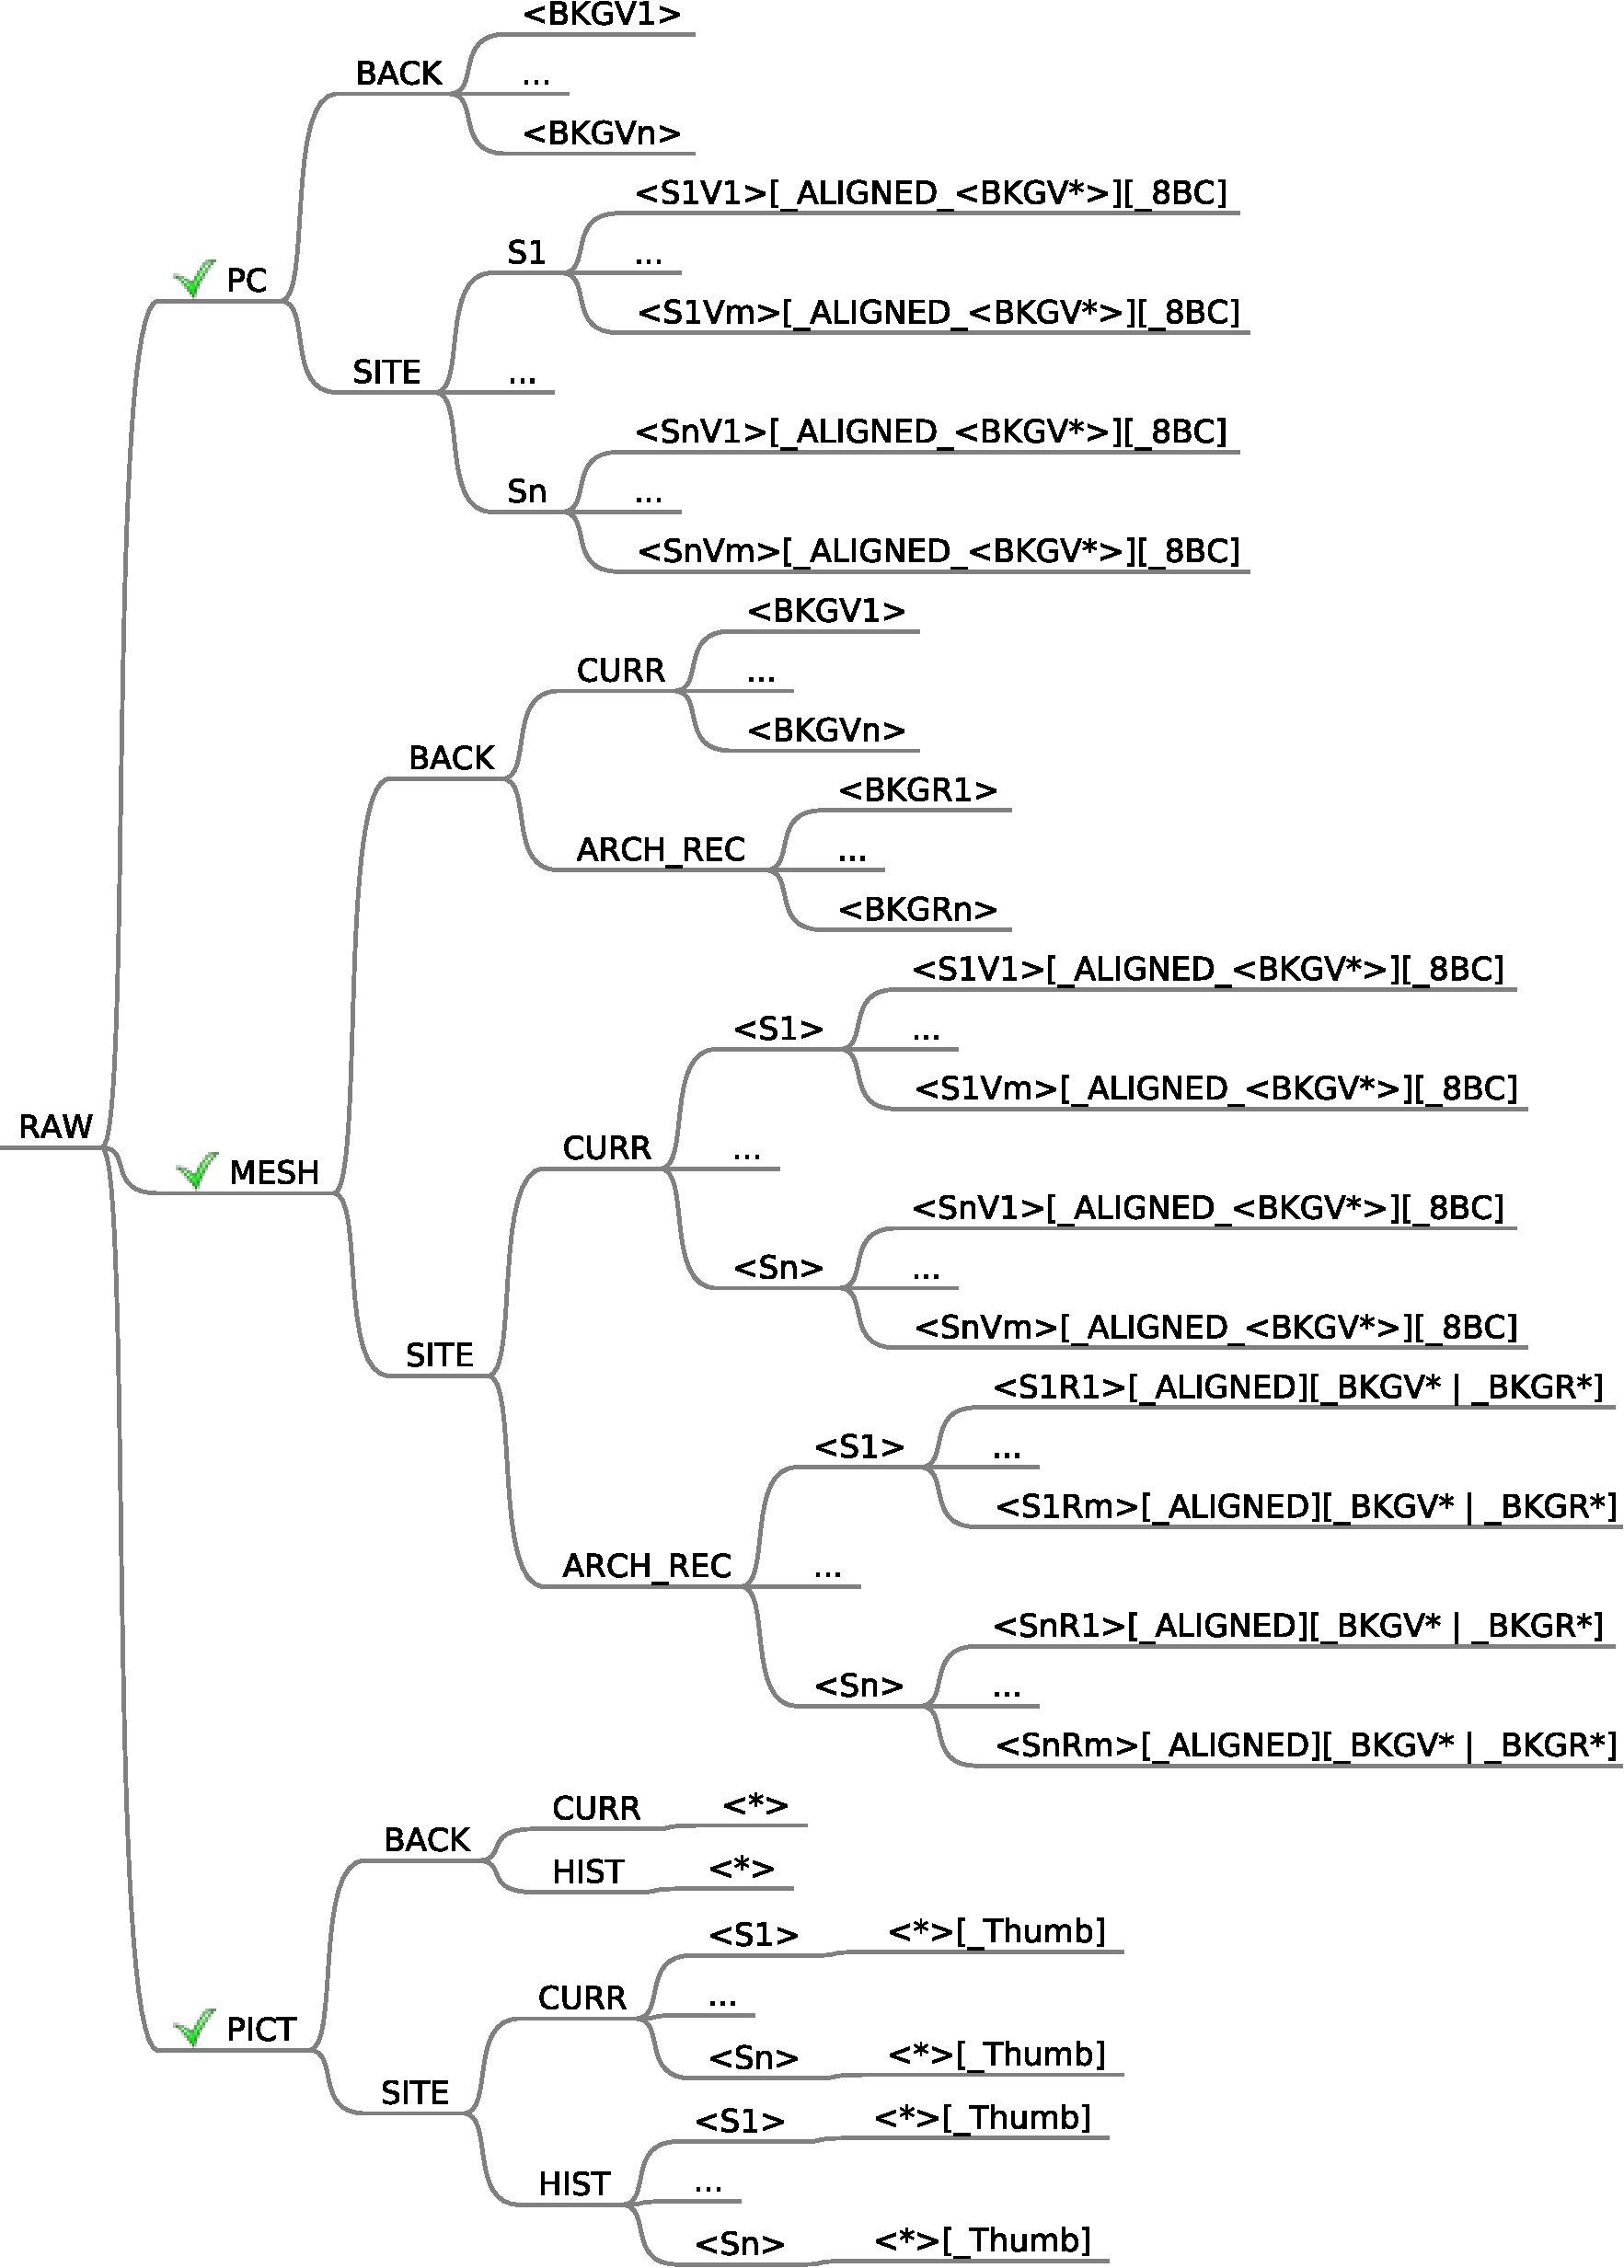
\includegraphics[width=0.8\textwidth]{fig/data_structure/directory_structure_raw}
\caption{Overview of the data structure: RAW data items}
\label{fig:directory_structure_overview_raw} \end{figure}


\subsection{Raw data management}
On the data structure it is possible to perform different operations. Such operations
are (1) adding raw data items (Section~\ref{sec:addraw}); (2) removing raw data
items (Section~\ref{sec:removeraw}); and (3) listing raw data items (Section~\ref{sec:listraw}).

\subsubsection{Adding raw data items}
\label{sec:addraw} 
The script \textit{AddRawDataItem.py} is used to add raw data items to the directory
structure. To run the script, the user needs, depending on the exact datatype,
to supply additional arguments to the script. An overview of the possible arguments
are found in the verbatim below. The script automatically creates a destination
folder with the required naming, as specified in section \ref{sec:descriptiondata},
using the supplied arguments.

For MESH and PICT, the (\textit{-f, -\hspace{0cm}-file}) argument can be either
a file, or a folder containing files with the correct extension. For a PC the
argument must always be a folder.

\begin{Verbatim}[fontfamily=courier,commandchars=\\\{\},fontsize=\footnotesize]
usage: AddRawDataItem.py [-h] [-i DATA] -k {BACK,SITE} -t {PC,MESH,PICT} -f
FILE
[-p {CURR,HIST,ARCH_REC}] [-s SRID] [--eight] [-l
{debug,info,warning,error,critical}] [--site SITE]

Add Raw data item to the file structure.

optional arguments: -h, --help            show this help message and exit -i
DATA, --data DATA  RAW data folder [default /home/pattydat/DATA/RAW] -s SRID,
--srid SRID  spatial reference system SRID [only for MESH SITE] --eight
8 bit color [only for PC SITE or MESH] -l {debug,info,warning,error,critical},
--log {debug,info,warning,error,critical} Log level

required arguments: -k {BACK,SITE}, --kind {BACK,SITE} Type of item -t
{PC,MESH,PICT}, --type {PC,MESH,PICT} Type of data -f FILE, --file FILE  Input
file/directory name to copy

required arguments for MESH and PICT: -p {CURR,HIST,ARCH_REC}, --period
{CURR,HIST,ARCH_REC} Period (choose from MESH:CURR,ARCH_REC; PICT:CURR,HIST)

required arguments for SITE: --site SITE           Site number \end{Verbatim}

\subsubsection{Removing raw data items}
\label{sec:removeraw} 
The \textit{RemoveRawDataItem.py} is used to remove raw data items from the file
structure. 
\begin{Verbatim}[fontfamily=courier,commandchars=\\\{\},fontsize=\footnotesize]
usage: RemoveRawDataItem.py [-h] -i ITEMID [-d DBNAME] [-u DBUSER] [-p DBPASS]
[-t DBHOST] [-r DBPORT] [-l {debug,info,warning,error,critical}]

Removes a list of Raw data items and their related converted data from the file
structure.

optional arguments: -h, --help            show this help message and exit -d
DBNAME, --dbname DBNAME PostgreSQL DB name viaappiadb] -u DBUSER, --dbuser
DBUSER DB user [default ronald] -p DBPASS, --dbpass DBPASS DB pass -t DBHOST,
--dbhost DBHOST DB host -r DBPORT, --dbport DBPORT DB port -l
{debug,info,warning,error,critical}, --log {debug,info,warning,error,critical}
Log level

required arguments: -i ITEMID, --itemid ITEMID Comma-separated list of Raw Data
Item Ids Raw data item id (with ? the available raw data items are listed)
\end{Verbatim}

\subsubsection{Listing raw data items}
\label{sec:listraw} 
The script \textit{ListRawDataItem.py} lists the raw data items currently in the
file structure.
\begin{Verbatim}[fontfamily=courier,commandchars=\\\{\},fontsize=\footnotesize]
usage: ListRawDataItem.py [-h] [-i ITEMID] [-d DBNAME] [-u DBUSER] [-p DBPASS]
[-t DBHOST] [-r DBPORT] [-l {debug,info,warning,error,critical}]

List the Raw data items that are in the DB.

optional arguments: -h, --help            show this help message and exit -i
ITEMID, --itemid ITEMID List the Raw Data Item Ids related to a list of items
(comma-separated) [default list all raw data items] -d DBNAME, --dbname DBNAME
PostgreSQL DB name viaappiadb] -u DBUSER, --dbuser DBUSER DB user [default
$USERNAME] -p DBPASS, --dbpass DBPASS DB pass -t DBHOST, --dbhost DBHOST DB
host -r DBPORT, --dbport DBPORT DB port -l {debug,info,warning,error,critical},
--log {debug,info,warning,error,critical} Log level

\end{Verbatim}

\subsubsection{Generating OSG data}
\label{sec:generateosg}
The script should be run with the \textit{vadata} user and should be run when some data has
changed in the raw data directory. The Potree data is copied automatically in
the Potree data tree, with the naming as specified in figure
\ref{fig:directory_structure_overview_osg}.
 
\begin{figure}[] \centering
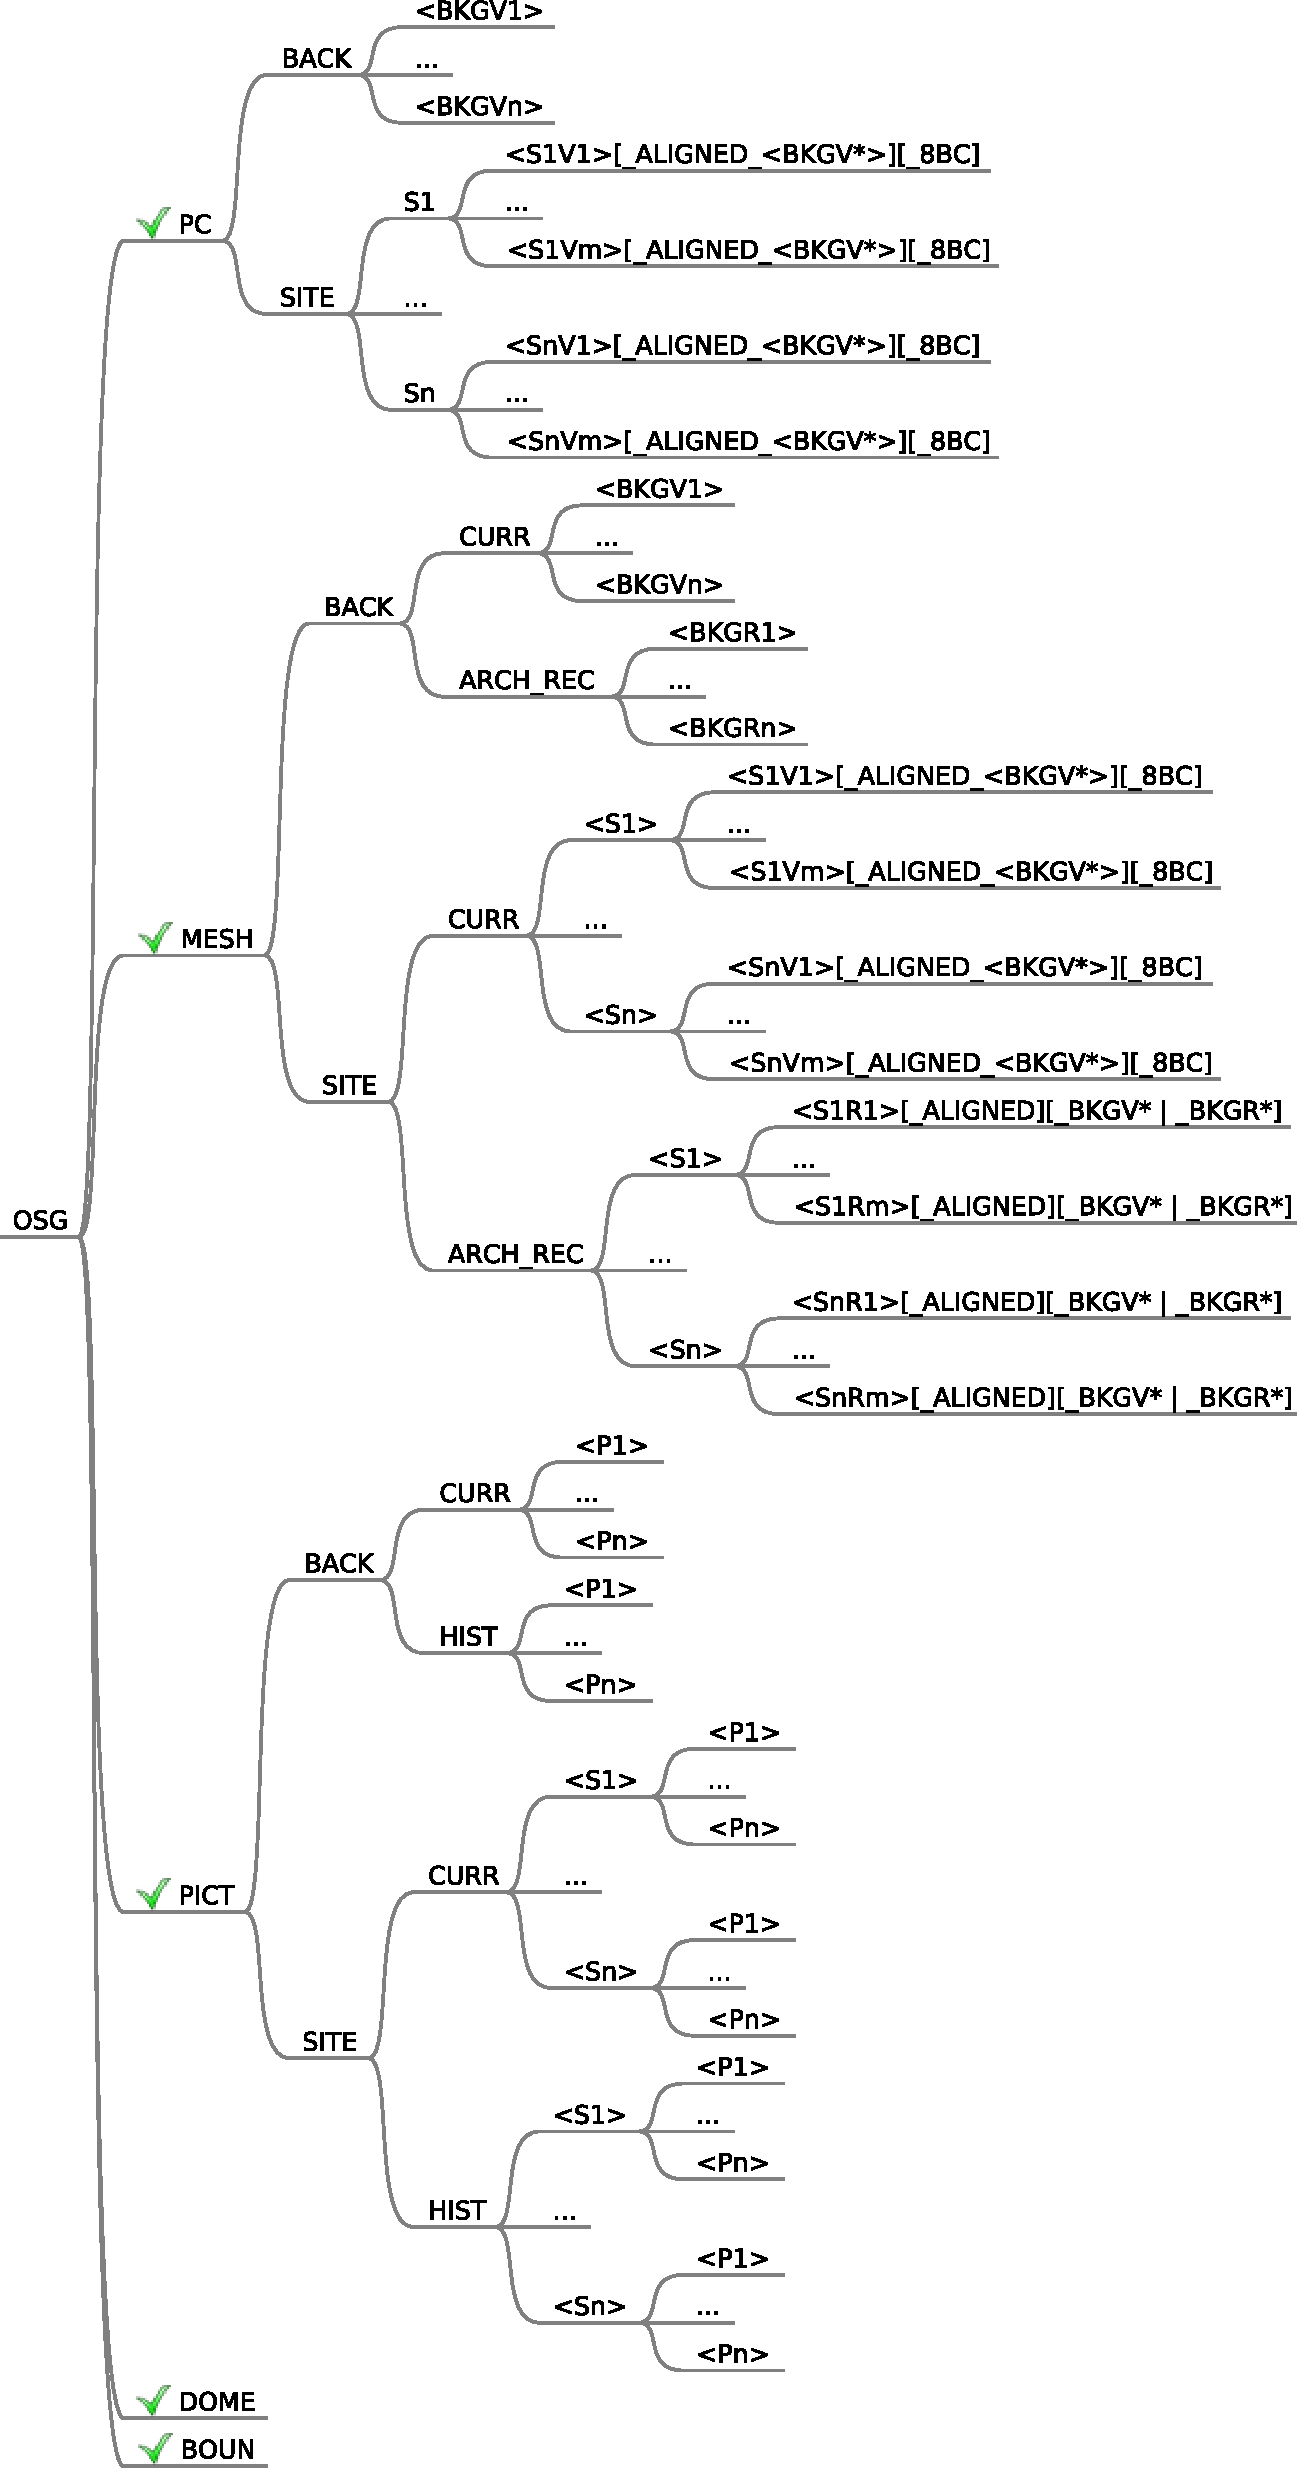
\includegraphics[width=0.7\textwidth]{fig/data_structure/directory_structure_osg}
\caption{Overview of the data structure: OSG data items}
\label{fig:directory_structure_overview_osg} \end{figure}

\begin{Verbatim}[fontfamily=courier,commandchars=\\\{\},fontsize=\footnotesize]
usage: GenerateOSG.py [-h] [-i ITEMID] [-d DBNAME] [-u DBUSER] [-p DBPASS] [-t
DBHOST] [-r DBPORT] [-o OSGDIR] [-l {debug,info,warning,error,critical}]

Generates the OSG data for a raw data item.

optional arguments: -h, --help            show this help message and exit -i
ITEMID, --itemid ITEMID Comma-separated list of Raw Data Item Ids [default is
to convert all raw data items related to sites that do not have a related OSG
data item] (with ? the available raw data items are listed, with ! the list all
the raw data items without any related OSG data item) -d DBNAME, --dbname
DBNAME Postgres DB name [default viaappiadb] -u DBUSER, --dbuser DBUSER DB user
[default $USERNAME] -p DBPASS, --dbpass DBPASS DB pass -t DBHOST, --dbhost
DBHOST DB host -r DBPORT, --dbport DBPORT DB port -o OSGDIR, --osgDir OSGDIR
OSG data directory [default /home/pattydat/DATA/OSG] -l
{debug,info,warning,error,critical}, --log {debug,info,warning,error,critical}
Log level \end{Verbatim}

\subsubsection{Generating Potree data}
\label{sec:generatePotree} 
The script should be run with the \textit{vadata} user and should be run when some data
has changed in the raw data directory. The Potree data is copied automatically
in the Potree data tree, with the naming as specified in figure
\ref{fig:directory_structure_overview_potree}.

\begin{figure}[] \centering
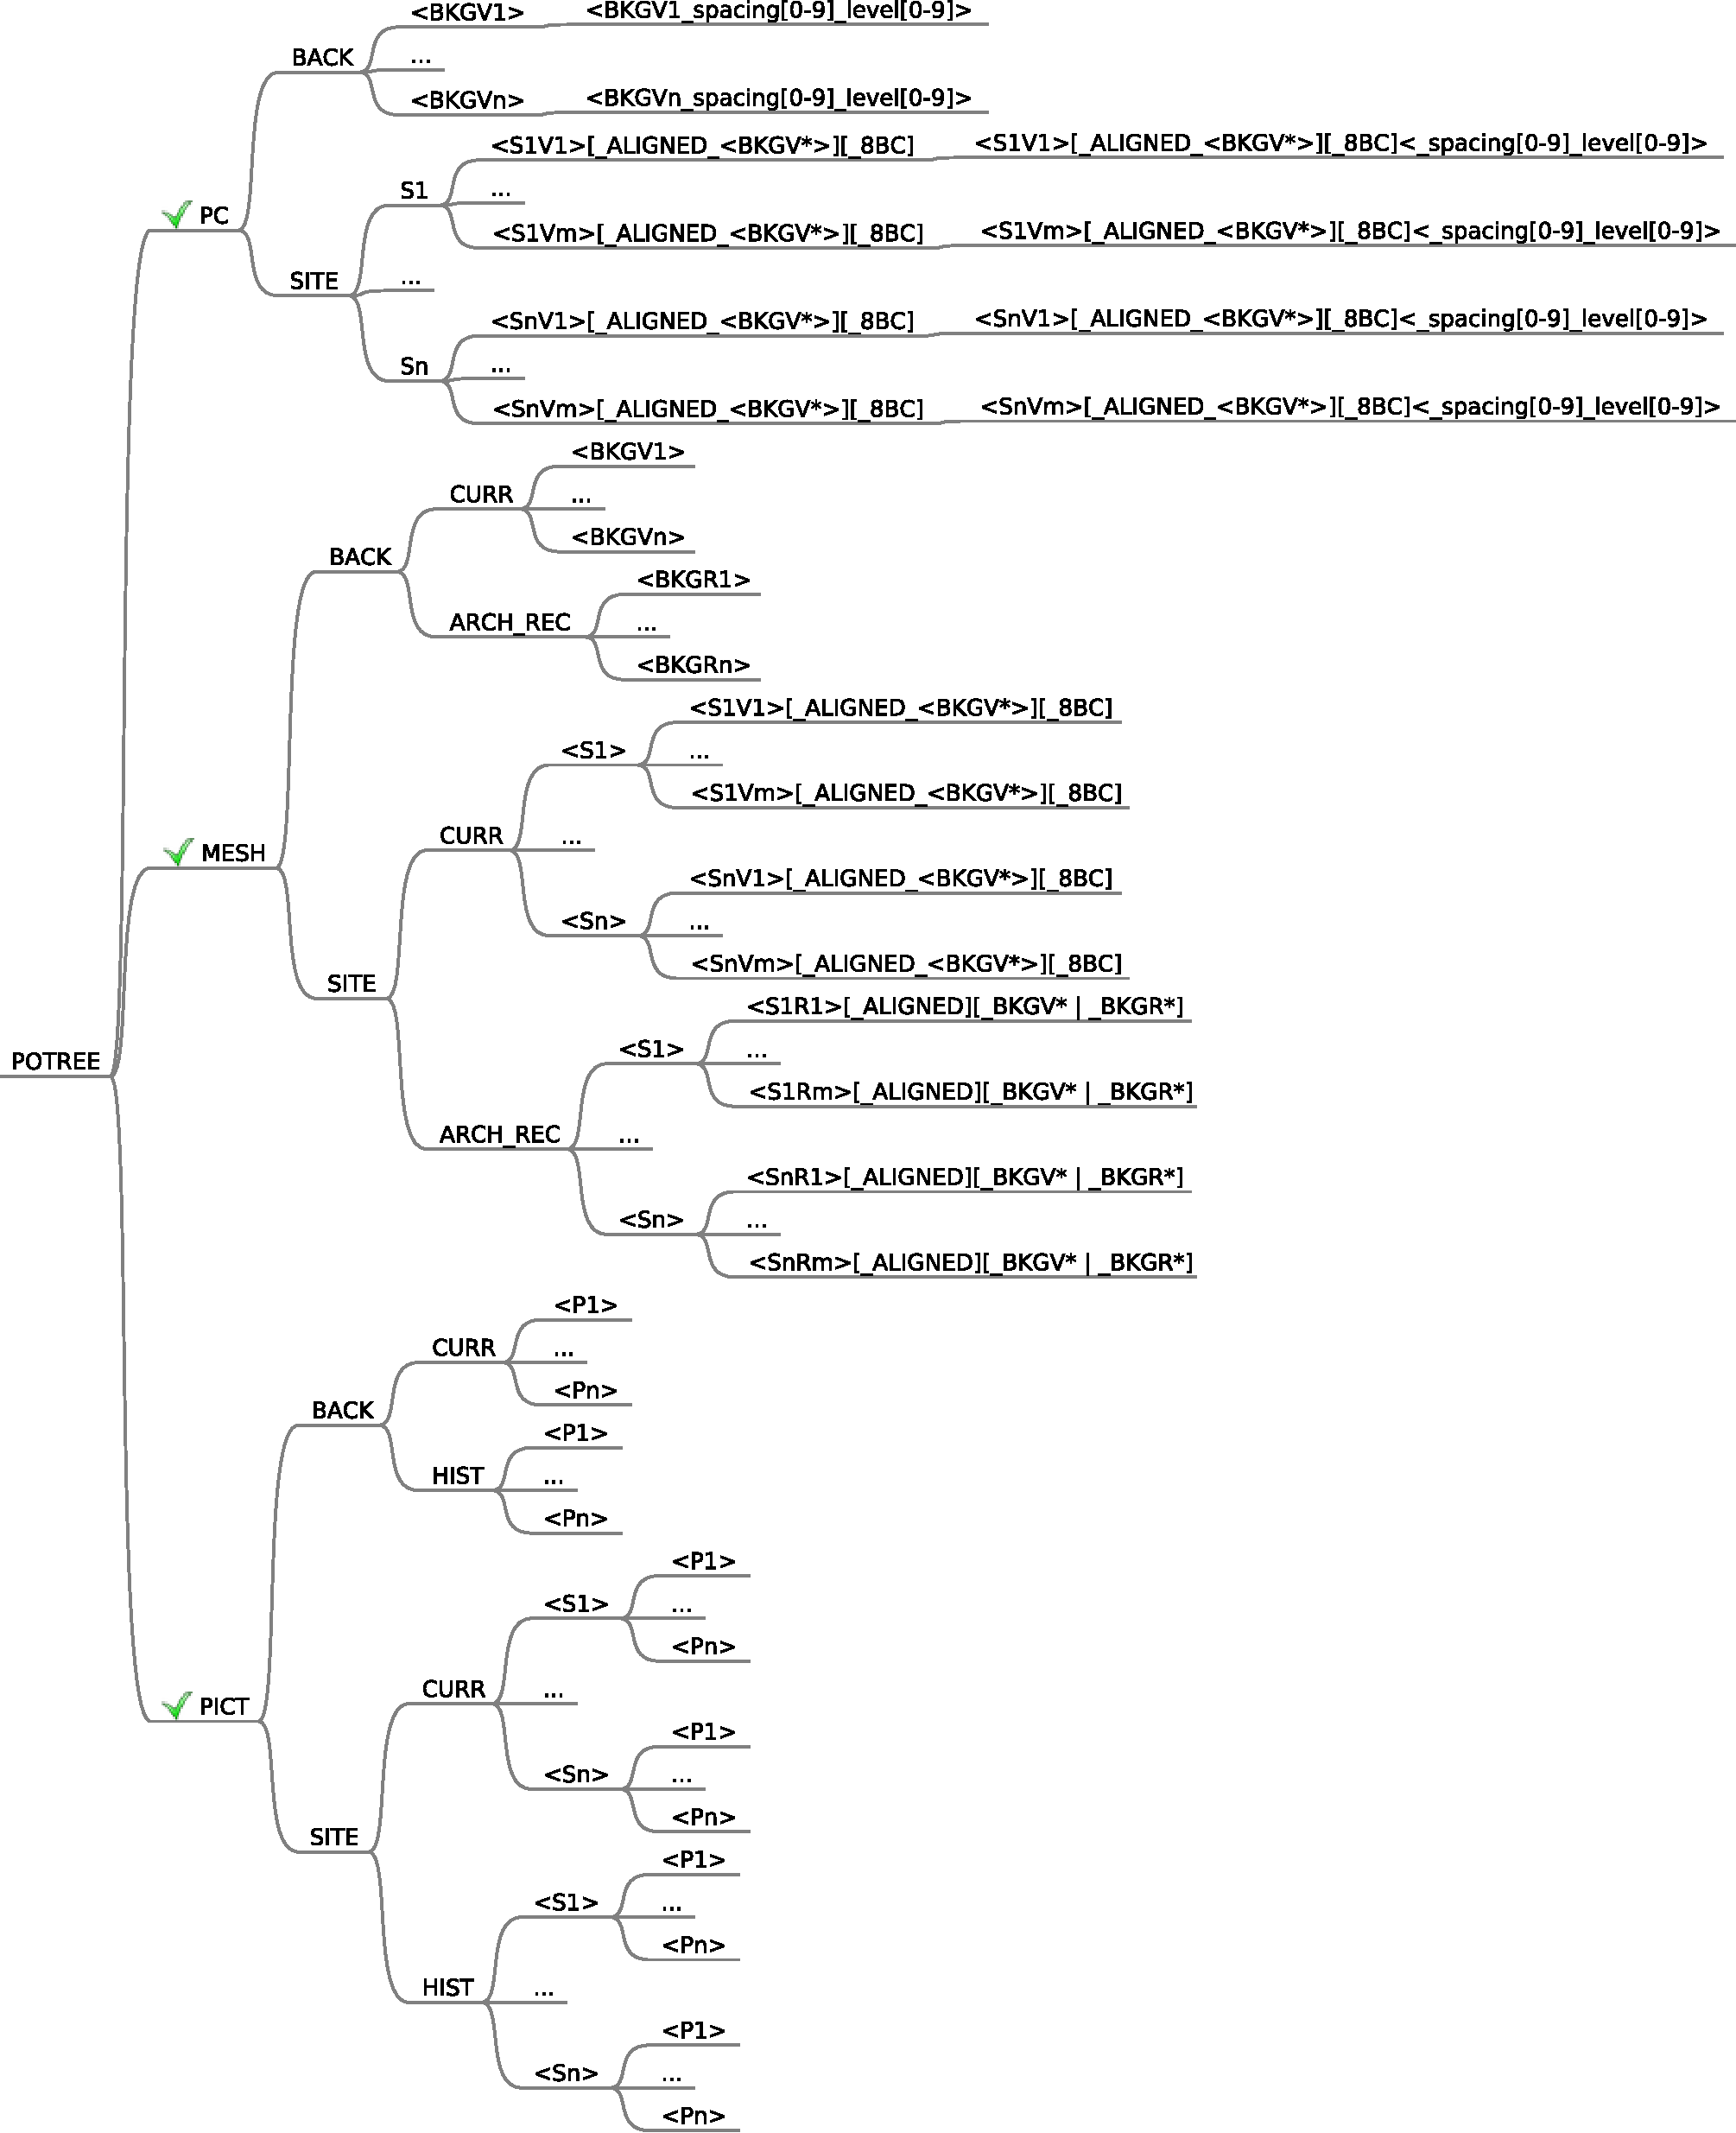
\includegraphics[width=1\textwidth]{fig/data_structure/directory_structure_potree}
\caption{Overview of the data structure: Potree data items}
\label{fig:directory_structure_overview_potree} \end{figure}

\begin{Verbatim}[fontfamily=courier,commandchars=\\\{\},fontsize=\footnotesize]
usage: GeneratePotree.py [-h] [-i ITEMID] [-d DBNAME] [-u DBUSER] [-p DBPASS]
[-t DBHOST] [-r DBPORT] [-o POTREEDIR] [--levels LEVELS] [-l
{debug,info,warning,error,critical}]

Generates the Potree data for a raw data item (ONLY FOR PCs)

optional arguments: -h, --help            show this help message and exit -i
ITEMID, --itemid ITEMID Comma-separated list of PointCloud Raw Data Item Ids
[default is to convert all raw data items that do not have a related Potree
data item] (with ? the available raw data items are listed, with ! the list all
the raw data items without any related Potree data item) -d DBNAME, --dbname
DBNAME Postgres DB name [default viaappiadb] -u DBUSER, --dbuser DBUSER DB user
[default $USERNAME] -p DBPASS, --dbpass DBPASS DB pass -t DBHOST, --dbhost
DBHOST DB host -r DBPORT, --dbport DBPORT DB port -o POTREEDIR, --potreeDir
POTREEDIR POTREE data directory [default /home/pattydat/DATA/POTREE] --levels
LEVELS       Number of levels of the Octree, parameter for PotreeConverter.
[default is 4 for Sites and 8 for Backgrounds] -l
{debug,info,warning,error,critical}, --log {debug,info,warning,error,critical}
Log level \end{Verbatim}
